% !TEX encoding = UTF-8
% !TEX TS-program = pdflatex
% !TEX root = ../tesi.tex

%**************************************************************
\chapter{Volume Rendering e Qt}
\label{cap:teoria-stage}
%**************************************************************

%**************************************************************
\section{Radiologia e rendering}
\intro{Concetti di base, teoria, algoritmi e gestione/caricamento immagini DICOM}\\

\subsection{Visualizzare informazioni}\label{sec:visualizzare-informazioni}
Visualizzare fa parte della nostra vita quotidiana: dalle mappe satellitari alla computer grafica dell'industria dell'intrattenimento, possiamo trovare esempi di visualizzazione praticamente ovunque. Ma che cosa significa visualizzare informazioni? Informalmente, visualizzare è la trasformazione di dati o informazioni in immagini. Visualizzare coinvolge la vista e la potenza di elaborazione della mente, con un risultato semplice ed efficace per comunicare informazioni complesse e/o voluminose.
\\
Tuttavia, forse la migliore definizione di visualizzazione si trova negli esempi. In molti casi la visualizzazione sta influenzando la vita delle persone e compiendo imprese che alcuni anni fa sarebbero state inimmaginabili, come nella medicina moderna, ambito su cui ci concentreremo.

\subsection{Volumi radiologici}\label{sec:volumi-radiologici}
Le tecniche di diagnostica per immagini, soprattutto in radiologia, sono diventate un importante strumento nella medicina moderna. Ci concentreremo su tecniche come la tomografia computerizzata (TC) e la risonanza magnetica (RM).
\\
Queste tecniche utilizzano dei processi di acquisizione e campionamento per raccogliere informazioni sull'anatomia interna di un paziente. Queste informazioni sono raccolte in forma di piani di taglio o in immagini in sezione trasversale di un paziente, in maniera simile a come accade per radiografie a raggi X convenzionali. La TC utilizza un fascio di raggi X per acquisire i dati, mentre la RM utilizza un forte campo magnetico unito a  impulsi a radiofrequenza. Varie tecniche matematiche vengono utilizzate per ricostruire i piani di taglio da salvare, dopodiché solitamente, questi vengono raccolte in un volume di dati.
\\
Un'immagine radiologica, o una fetta del volume nel nostro caso, è acquisita come una serie di valori che rappresenta l'attenuazione dei raggi X (nella TC) o il rilassamento dello spin di un atomo. Ogni immagine contiene tutti questi dati in un array, o in una matrice, tuttavia la quantità di dati è così grande che è impossibile comprenderli nella loro forma "grezza". Per questo, assegnandogli una scala di grigi e visualizzandoli su uno schermo, si riesce finalmente a visualizzare la struttura, permettendoci di visualizzare ciò che il computer vede come un insieme di valori come una sezione del corpo umano.

\subsection{Basi di rendering}\label{sec:basi-rendering}
La computer grafica è il processo di generare immagini utilizzando il computer, questo processo viene chiamato rendering. Ci sono molti tipi di rendering, dal disegno 2D a tecniche 3D sofisticate. In questa sezione vedremo le basi del rendering 3D.
\\
Nel mondo reale quando guardiamo un oggetto, per esempio una scatola, i raggi di luce emessi da una sorgente luminosa (per esempio il sole) sono emessi in tutte le direzioni. Alcuni di questi colpiscono la scatola che ne assorbe una parte di luce e ne riflette il resto. Una parte di questa luce riflessa potrebbe dirigersi verso di noi ed entrare nei nostri occhi, se questo succede noi riusciamo a vedere l'oggetto. Allo stesso modo se della luce colpisce il terreno una parte si rifletterà nei nostri occhi.

\begin{figure}[h]
    \centering
    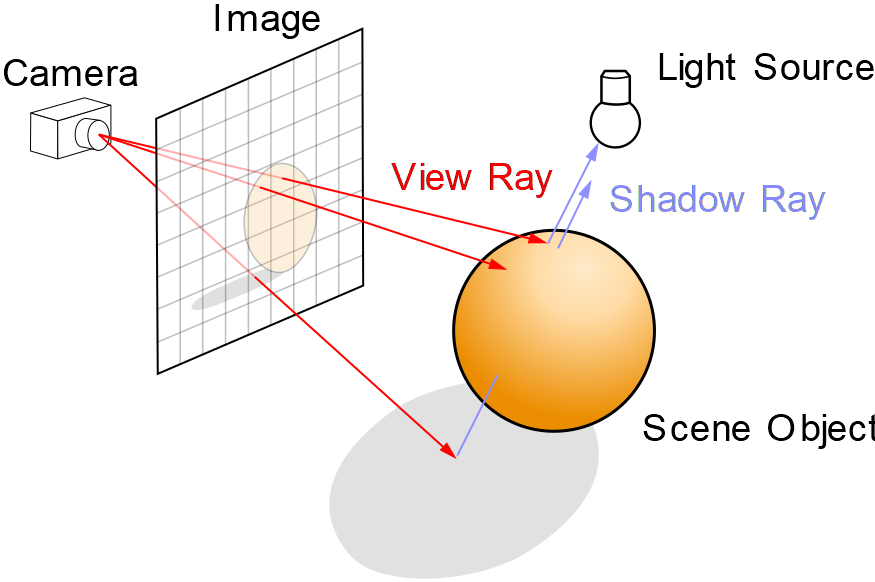
\includegraphics[width=0.5\textwidth]{immagini/volumerendering/ray_tracing_diagram.png}
    \caption{\textit{Algoritmo di Ray-Tracing}}
    \textbf{Fonte}: \href{https://en.wikipedia.org/wiki/Ray_tracing_(graphics)}{wikipedia.org/wiki/Ray\_tracing}
    \label{fig: Algoritmo di Ray-Tracing}
\end{figure}

Una tecnica comune ed efficace per la computer grafica 3D è il ray-tracing, a volte chiamata anche ray-casting. Il ray-tracing simula l'interazione della luce con gli oggetti, seguendo il percorso di ogni raggio. Di solito, si segue il raggio dall'indietro, dalla posizione dell'osservatore (la camera nello schema) nel mondo per determinare che cosa il raggio colpisce. La direzione del raggio quindi, è la direzione che si sta osservando. Quando un raggio colpisce un oggetto, possiamo determinare se quel punto è illuminato da una sorgente di luce: questo viene fatto tracciando un raggio dal punto di intersezione alla luce: se il raggio colpisce qualcos'altro prima di raggiungere la sorgente luminosa, allora quella luce non contribuirà a illuminare il punto. Se ci sono N sorgenti luminose, questo andrà fatto per ognuna di esse.
\\
Per chi non avesse mai sentito parlare del ray-tracing, sarà sorprendente scoprire che non è quasi mai usato nella grafica real-time. Questo perchè il ray-tracing è un processo molto lento e dispendioso in termini di risorse, oltre al fatto che fino a pochi anni fa era possibile implementarlo solo via software, per questo sono state sviluppate altre tecniche che generano immagini sfruttando meglio l'accelerazione hardware.
\\
La spiegazione fino a questo punto ha assunto che stessimo facendo il render di un oggetto solido. Tuttavia, oggetti come nuvole, l'acqua, la nebbia sono "traslucidi" o diffondono la luce che li attraversa, questi oggetti non possono essere renderizzati utilizzando esclusivamente le interazioni sulle superfici. Dobbiamo invece considerare le proprietà mutevoli all'interno dell'oggetto per mostrarlo correttamente. Ci riferiamo quindi a due modelli di rendering:
\begin{itemize}
\item surface rendering: esegue il render della superficie di un oggetto;
\item volume rendering: esegue il rendering della superficie e dell'interno di un oggetto.
\end{itemize}

Le tecniche di volume rendering ci consentono di vedere la "disomogeneità" all'interno degli oggetti. Nella TC per esempio, possiamo riprodurre realisticamente immagini a raggi X considerando i valori di intensità sia sulla superficie che all'interno. Vedremo più dettagli sul volume rendering nella prossima sezione, ma tornando all'esempio del ray-tracing, si può immaginare come i raggi non interagiscano solo con la superficie di un oggetto, ma anche con ciò che è al suo interno.

%**************************************************************
\section{Volume rendering}
\subsection{Basi di volume rendering}\label{sec:volume-rendering-details}
Finora ci siamo concentrati sulla visualizzazione di dati tramite l'utilizzo di primitive come punti, linee e poligoni. Per molte applicazioni questo è chiaramente il metodo migliore per rappresentarli, tuttavia alcune applicazioni ci richiedono di visualizzare dati che sono "volumetrici", più comunemente chiamati immagini 3D o set volume di dati (volume datasets). Per esempio, nell'imaging biomedico potremmo aver bisogno di visualizzare dati ottenuti da una RM, una TC, un microscopio o un'ecografia. Anche l'analisi meteorologica e altre simulazioni producono grandi quantità di dati volumetrici in tre o più dimensioni che richiedono tecniche di visualizzazione efficaci.
\\
Vedremo ora più in dettaglio alcuni metodi di volume rendering che usano...?
\\
Considerando che il rendering volumetrico è tipicamente usato per generare immagini che rappresentano un intero set 3D in un'immagine 2D, bisogna prestare attenzione ad alcuni punti: una classificazione deve essere eseguita per assegnare colore e opacità alle regioni all'interno del volume, e devono essere definite delle tecniche di illuminazione volumetrica per migliorare il risultato.

\subsection{Volume rendering Image-Order}\label{sec:volume-image-order}
Il volume rendering Image-Order è spesso chiamato "ray casting" o "ray tracing". L'idea di base è determinare il valore di ogni pixel dell'immagine, inviando un raggio dalla posizione del pixel nella scena, secondo i valori della visuale corrente. A quel punto si  valutano i dati incontrati lungo il raggio, per calcolare il valore del pixel. Come vedremo, il ray casting è una tecnica che può essere usata per fare il render di qualsiasi dataset 3D producendo una grande varietà di immagini, ed è relativamente semplice estenderlo in modo da utilizzarlo per un set di dati volumetrici per lavorare su "griglie" ben strutturate. Sfortunatamente, il ray casting è un processo abbastanza lento, pertanto si utilizzano una serie di metodi di accelerazione per migliorare le prestazioni, sacrificando alcuna memoria aggiuntiva o parte di flessibilità dell'algoritmo.

\begin{figure}[h]
    \centering
    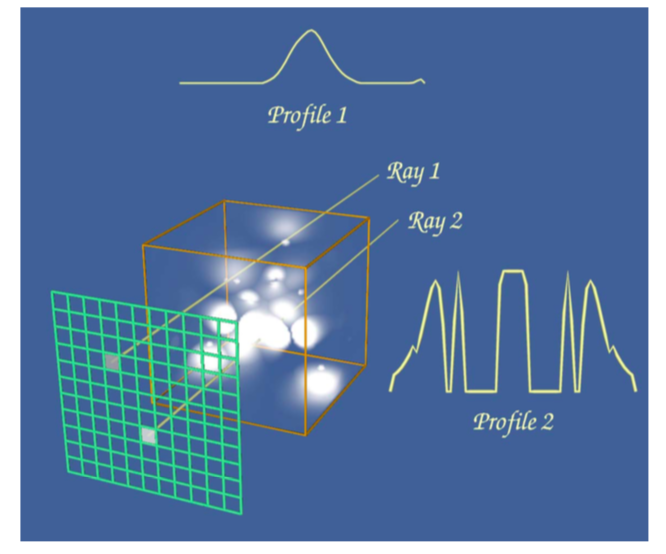
\includegraphics[width=0.5\textwidth]{immagini/volumerendering/imageorder.png}
    \caption{\textit{Volume Rendering Image-Order}}
    \textbf{Fonte}: \href{https://lorensen.github.io/VTKExamples/site/VTKBook/07Chapter7/}{VTKBook/Chapter7/}
    \label{fig: Volume Rendering Image-Order}
\end{figure}

Un esempio del processo di ray casting è illustrato nell'immagine qui sopra. Questo esempio utilizza una proiezione ortografica della camera standard, di conseguenza tutti i raggi sono paralleli l'un l'altro e perpendicolari alla vista (anche chiamata "view plane"). I dati processati lungo ciascun raggio sono processati con una funzione specifica, che in questo caso determina il valore massimo incontrato e lo converte ad una scala di grigi, dove il valore minimo è mappato come nero trasparente, e il massimo valore è mappato come bianco opaco.

\subsection{Volume rendering Object-Order}\label{sec:volume-object-order}
Il volume rendering Object-Order processa i valori nel volume basandosi sull'organizzazione dei voxel nel dataset e sulle impostazioni della visuale corrente. Quando un metodo "alpha compositing" è utilizzato, i voxel vanno processati in ordine "front-to-back" o "back-to-front" per ottenere risultati corretti. Se si sfrutta l'hardware dedicato, è preferibile utilizzare l'ordine "back-to-front" in quanto si evita di calcolare dei valori extra riguardo la trasparenza. Al contrario, se si utilizza il render software, l'ordine "front-to-back" è più comune in quanto è possibile evitare di processare ulteriori dati quando un pixel raggiunge la "piena opacità". Alcune tecniche, come la MIP, possono essere processate in qualsiasi ordine per ottenere risultati corretti.

\begin{figure}[h]
    \centering
    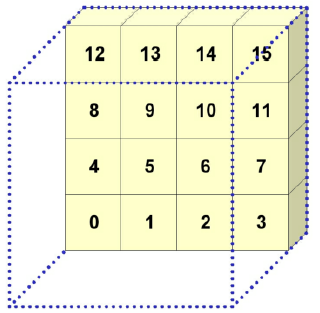
\includegraphics[width=0.5\textwidth]{immagini/volumerendering/objectorder.png}
    \caption{\textit{Volume Rendering Object-Order}}
    \textbf{Fonte}: \href{https://lorensen.github.io/VTKExamples/site/VTKBook/07Chapter7/}{VTKBook/Chapter7/}
    \label{fig: Volume Rendering Object-Order}
\end{figure}

La figura qui sopra rappresenta un approccio "back-to-front" per calcolare i voxel: si parte dal voxel più lontano rispetto alla visuale, e si prosegue visitandoli in ordine di distanza finchè non sono stati tutti visitati.

\subsection{Funzione di trasferimento}\label{sec:funzione-trasferimento}
Una funzione di trasferimento è responsabile della mappatura delle informazioni dei voxel in valori differenti come materiale, colore o trasparenza. Uno dei punti di forza del volume rendering, è che può gestire funzioni di trasferimento di complessità molto maggiore di una funzione "a passo binario". Questo è spesso necessario considerando che i dataset contengono più materiali e un metodo di classificazione non può sempre riuscire ad assegnare un singolo materiale ad un campione.

\begin{figure}[h]
    \centering
    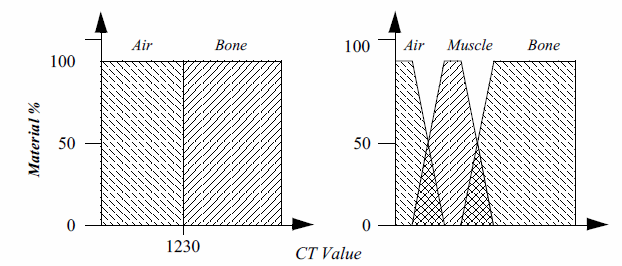
\includegraphics[width=0.5\textwidth]{immagini/volumerendering/functions.png}
    \caption{\textit{Semplice classificazione binaria (sinistra) e una transizione graduale tra aria a muscoli a ossa (destra).}}
    \textbf{Fonte}: \href{https://lorensen.github.io/VTKExamples/site/VTKBook/07Chapter7/}{VTKBook/Chapter7/}
    \label{fig: Volume Rendering Object-Order}
\end{figure}

Prendendo come esempio una TC, ora possiamo specificare una funzione di trasferimento che definisca una transizione graduale da aria, a muscoli, ad ossa, come mostrato nell'immagine qui sopra.

Altro???

\subsection{Regioni di interesse}\label{sec:regioni-di-interesse}
Un problema nel visualizzare dati volumetrici, è che se volessi studiare alcuni dati al centro del volume, dovrei guardare a tutto ciò che c'è attorno nel dataset. Per esempio, se visualizzassi il dataset di un pomodoro, non riuscirei a vedere i semi perché con tecniche come la MIP, vedrei tutta la polpa circostante.

\begin{figure}[h]
    \centering
    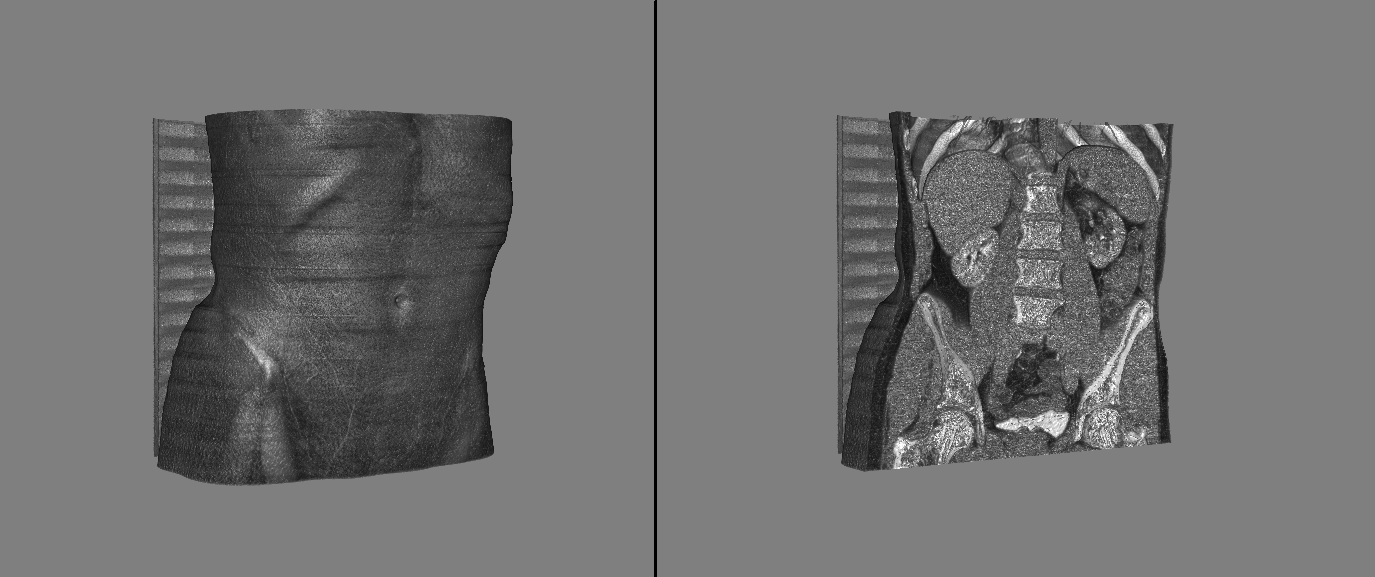
\includegraphics[scale=0.3]{immagini/volumerendering/regionofinterest.png}
    \caption{\textit{Esempio di volume rendering con regione di interesse, tagliando il volume.}}
    \textbf{Fonte}: Stage
    \label{fig: Volume Rendering con Regione di Interesse}
\end{figure}

Possiamo risolvere questo problema di visualizzazione interna, definendo una regione di interesse del nostro volume, e facendo il render quindi solo di una porzione del dataset come mostrato nella figura qui sopra. Ci sono molte tecniche per definire una regione di interesse: si potrebbe utilizzare i piani "far" e "near" della camera per escludere parti del volume; altrimenti si possono definire sei piani (un cubo quindi) per definire un sotto-volume da visualizzare, escludendo il resto all'esterno del cubo; si possono anche utilizzare più piani distinti per escludere sezioni in varie posizioni e orientamenti.

%**************************************************************
\section{VTK}

\begin{figure}[h]
    \centering
    \includegraphics[scale=0.1]{immagini/volumerendering/VTK_logo.png}
    \caption{\textit{Logo di VTK}}
    \textbf{Fonte}: \href{https://vtk.org/}{vtk.org}
    \label{fig: Logo VTK}
\end{figure}

\subsection{Descrizione e scelta della libreria}\label{sec:scelta-liberia}
Il Visualization Toolkit (VTK) è un software open-source cross-platform per la computer grafica 3D, l'elaborazione delle immagini e la visualizzazione scientifica. VTK consiste in una libreria C++ e vari layer di interfaccia, per esempio per Java o Python. VTK è sviluppato e supportato dal team Kitware, lo stesso team che ha sviluppato CMake, lo strumento di build nominato in precedenza. VTK supporta vari algoritmi di visualizzazione, e oltre al framework di visualizzazione contiene gli strumenti per interagire in 3D con un oggetto, supporta l'elaborazione parallela e si integra con vari database e toolkit GUI come Qt.\\
La libreria è stata proposta dal tutor dello stage, che l'aveva studiata e provata in passato, e voleva approfondirne le capacità e le funzionalità.

\subsection{Build della libreria}\label{sec:build-liberia}
VTK non offre dei binari precompilati per utilizzare la libreria, per utilizzarla quindi, bisognerà compilarla manualmente nella propria macchina. Questo è utile anche perché permette di configurare i moduli necessari da compilare e quelli da escludere. Il modo più semplice e raccomandato per fare il build della libreria, è CMake, nato proprio per supportare lo sviluppo di VTK e ITK. Con CMake possiamo quindi, per esempio, escludere dalla compilazione la documentazione, gli esempi, CUDA e l'integrazione con Java e Python, tutti moduli non necessari per il nostro progetto, dobbiamo tuttavia specificare che vogliamo usare Qt, in modo da compilarne il modulo che lo supporta. Parleremo meglio di Qt nella sezione \nameref{sec:qt-integrazione}.\\
Una volta configurato e generato il progetto con CMake, sarà sufficiente compilarlo per ottenere i file libreria da utilizzare nel proprio progetto, configurando appositamente il linker C\texttt{++}.

\subsection{Oggetti di rendering}\label{sec:oggetti-rendering}
\begin{figure}[h]
    \centering
    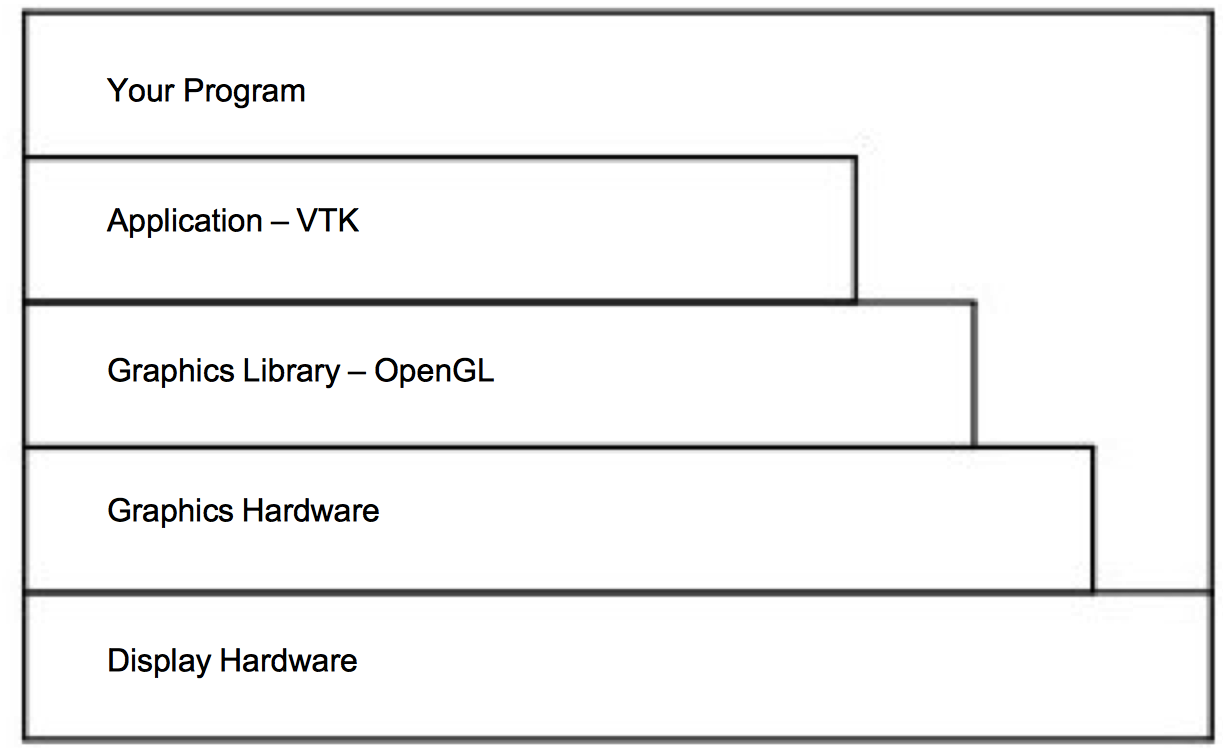
\includegraphics[scale=0.4]{immagini/volumerendering/layers.png}
    \caption{\textit{Gerarchia applicazione}}
    \textbf{Fonte}: \href{https://lorensen.github.io/VTKExamples/site/VTKBook/03Chapter3/}{VTKBook/Chapter3/}
    \label{fig: vtk-layers}
\end{figure}

Ora che abbiamo discusso le basi di rendering e di VTK, la buona notizia è che raramente dovremo preoccuparci di implementarle o modificarle. La maggior parte della programmazione grafica viene eseguita utilizzando primitive, la figura \ref{fig: vtk-layers} ci mostra la gerarchia di visualizzazione. Al primo posto c'è il nostro programma, e nei tre livelli sottostanti ci sono i livelli da tenere in considerazione.

\begin{figure}[h]
    \centering
    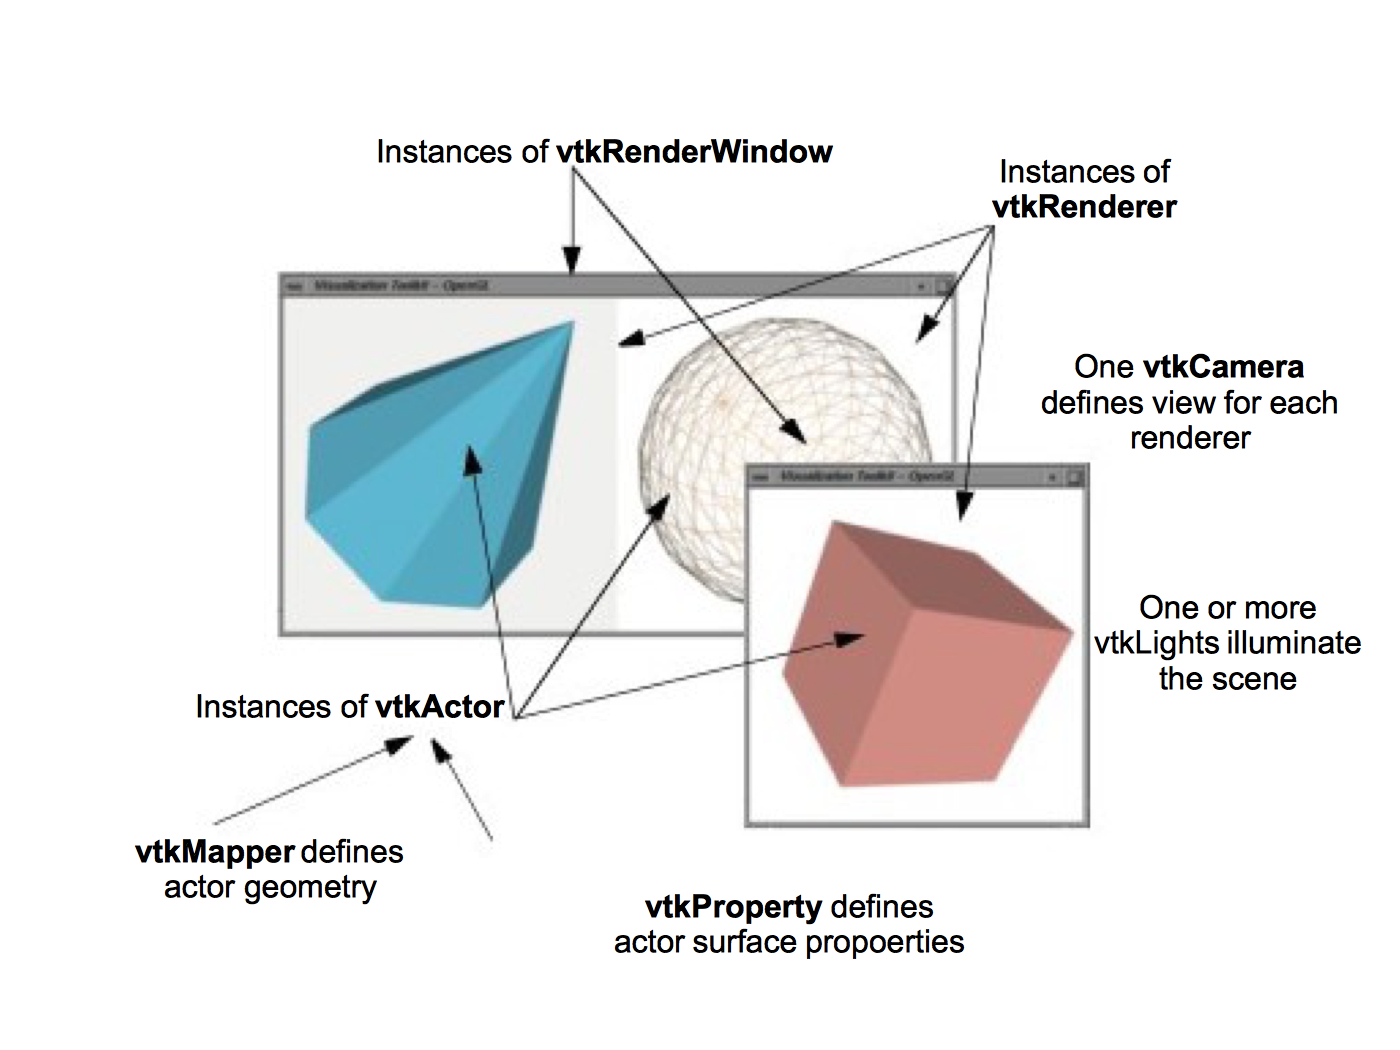
\includegraphics[scale=0.5]{immagini/volumerendering/vtkobjects.png}
    \caption{\textit{Oggetti di rendering di VTK}}
    \textbf{Fonte}: \href{https://lorensen.github.io/VTKExamples/site/VTKBook/03Chapter3/}{VTKBook/Chapter3/}
    \label{fig: Oggetti Rendering VTK}
\end{figure}

VTK contiene molti oggetti che utilizziamo per fare il render di una scena, molti sono dietro le quinte, ma vediamo i principali mostrati anche nella figura \ref{fig: Oggetti Rendering VTK}:
\begin{itemize}
\item vtkRenderWindow: gestisce una finestra sul dispositivo di visualizzazione, uno o più rendere disegnano in un'istanza di vtkRenderWindow;
\item vtkRenderer: controlla il processo di rendering degli oggetti, processando gli attori nella scena, le luci e la vista, in un'immagine;
\item vtkLight: una sorgente di luce che illumina la scena;
\item vtkCamera: definisce la posizione della vista, il punto focale, e altre proprietà di visualizzazione della scena;
\item vtkActor: rappresenta un oggetto nella scena di cui fare il render, comprese le sue proprietà e la sua posizione;
\item vtkProperty: definisce le proprietà di un attore, tra cui il colore, la trasparenza, e le proprietà luminose;  
\item vtkMapper: definisce la rappresentazione geometrica di un attore, più attori quindi possono riferirsi allo stesso vtkMapper.
\end{itemize}

\subsection{Altro?}\label{sec:aaa}

\subsection{Widget e interazione utente}\label{sec:widget-interazione}
Oltre a visualizzare vari elementi, l'interazione è una feature essenziale per permettere di analizzare meglio ciò che si sta mostrando. VTK contiene classi come vtkRenderWindowInteractor e vtkInteractorStyle che catturano eventi della finestra e li traducono in eventi utilizzabili da VTK, sono utili principalmente per manipolare la visuale o gli attori (per esempio ruotandoli) per ottenere una vista desiderata. Tuttavia questa funzionalità è abbastanza limitata riguardo l'interazione con i dati, non permettendoci per esempio di definire una regione di interesse.\\
Per questo sono stati introdotti i Widget 3D, che sono in grado di fornire la varietà di tecniche di interazione necessarie in un sistema di visualizzazione di questo tipo. In VTK gli eventi sono catturati da vtkRenderWindow, gli osservatori registrati ricevono gli eventi ed eseguono delle azioni: processando l'evento o passandolo ad un altro osservatore.

\begin{figure}[h]
    \centering
    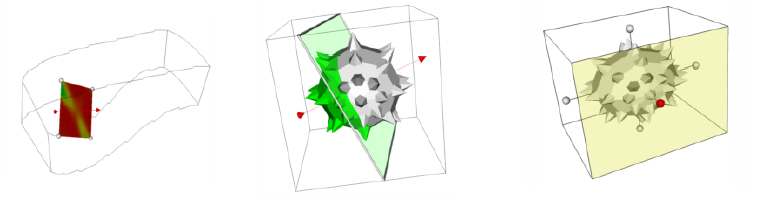
\includegraphics[scale=0.5]{immagini/volumerendering/widgets.png}
    \caption{\textit{Esempi di Widget 3D di VTK}}
    \textbf{Fonte}: \href{https://lorensen.github.io/VTKExamples/site/VTKBook/07Chapter7/}{VTKBook/Chapter7/}
    \label{fig: VTK 3D Widgets}
\end{figure}

Nella figura \ref{fig: VTK 3D Widgets} vediamo alcuni esempi di Widget 3D, in ordine un vtkPlaneWidget, vtkImplicitPlaneWidget e un vtkBoxWidget. \`E importante che i widget siano disegnati in modo da essere intuivi, per esempio i sei lati che delimitano il vtkBoxWidget sono rappresentati da sei piccole sfere, che possono essere selezionate e trascinate per ridimensionarlo.

%**************************************************************
\subsection{Integrazione con Qt}\label{sec:qt-integrazione}
Nel mio caso, dovevo utilizzare VTK con Qt, in modo da tenere Qt come libreria principale di gestione della UI. Il primo passo, come spiegato, è di compilare VTK con il supporto a Qt: questo richiede un'installazione già presente di Qt in modo da indicare a VTK quale versione e quali file di Qt utilizzare. Io ho utilizzato Qt 5.15, l'ultima versione disponibile.\\
Una volta impostato VTK, sarà quindi possibile creare un Widget Qt che deriva da QVTKOpenGLNativeWidget, ottenendo un Widget su cui è possibile mostrare il render effettuato da VTK.

%**************************************************************
\section{Strumenti CTK}
\begin{figure}[h]
    \centering
    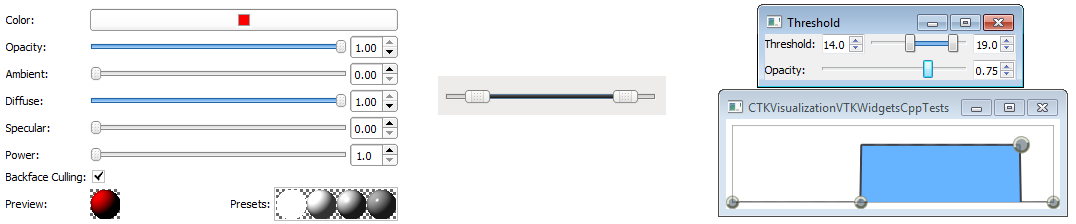
\includegraphics[scale=0.35]{immagini/volumerendering/ctkwidgets.png}
    \caption{\textit{Esempi di Widget 3D di CTK}}
    \textbf{Fonte}: \href{https://commontk.org/index.php/Documentation/ImageGallery}{commontk.org/Documentation}
    \label{fig: CTK 3D Widgets}
\end{figure}

Il "Common Toolkit" (CTK) è un una serie di strumenti di supporto per imaging medico e scopi correlati, come le applicazioni DICOM. Offre per esempio degli strumenti per interagire con i databse medicali DICOM, una serie di plugin e strumenti a riga di comando e una serie di Widget 3D per facilitare l'interazione con VTK, come si può vedere nell'immagine \ref{fig: CTK 3D Widgets}, in cui si vede un pannello per definire le proprietà dei materiali, un "double-range-slider" e un pannello per modificare le funzioni, in questo caso la funzione di threshold.
\\
Anche se la serie di strumenti offerti da CTK è stata studiata e analizzata, non è stata attivamente utilizzata come libreria durante lo stage.

%**************************************************************
\section{Basi di ITK}

Il "Insight Segmentation and Registration Toolkit" (ITK) è un framework open-source cross-platform, utilizzato per lo sviluppo di programmi di segmentazione, o "registrazione" (registration) immagini. La segmentazione è il processo di identificazione e classificazione dei dati trovati in una rappresentazione campionata digitalmente, nel nostro caso principalmente da un'immagine acquisita da strumentazione medica come scanner TC o RM. La registrazione è il compito di allineare o sviluppare corrispondenze tra i dati: ad esempio, in ambiente medico, una scansione TC può essere allineata con una scansione RM per combinare le informazioni contenute in entrambe.
\\
ITK era già nel piano di lavoro definita come una libreria da considerare solo opzionalmente per eventuali lavori futuri, e non è stata utilizzata durante lo stage.

%**************************************************************
\section{Software correlati}
Un software importante che è stato preso in considerazione durante lo stage è 3D Slicer, un software open source per l'analisi delle immagini e la visualizzazione scientifica, che fa amplio utilizzo di VTK, CTK e ITK. \`E stato preso come principale software di riferimento, sia per capire come utilizza VTK e le sue funzionalità, sia come fonte di ispirazione riguardo i tool necessari per interagire con un volume. Per esempio: la lista in formato XML dei Preset delle funzioni di trasferimento, è presa dal repository di 3D Slicer, e ne è stato fatto un parser apposito, considerando che sono funzioni standard usate in tutti i software di visualizzazione medica.\\
Per analizzare al meglio il funzionamento di 3D Slicer, ad inizio stage si era pensato di compilarlo dai sorgenti in modo da poterne effettuare il debug, tuttavia si è rivelato un processo molto arduo, in quanto la documentazione su come compilarlo non è sempre precisa, e fare un build con quasi tutti i moduli ha richiesto anche più di 6 ore su un processore Intel i7 di ultima generazione, dopo qualche tentativo quindi, l'idea è stata abbandonata in quanto non strettamente necessaria.

